\documentclass[acmtog]{acmart}
\usepackage{graphicx}
\usepackage{subfigure}
% Title portion
\title{Assignment 1 : Creating your own OpenGL program} 
\author{Name:\quad Chenghua Yang  \\ student number:\quad 2019533089
	\\email:\quad yangchh@shanghaitech.edu.cn}

\parindent=50pt
% Document starts
\begin{document}
\maketitle

\vspace*{2 ex}


\section{Introduction}
\subsection{Hi}
    Hi, this is my 1st HW of CS17.01.\\
    To see my \textbf{code}, please check the \texttt{VS2019 solution} in the \textbf{build} folder.\\
    To see my result, please unzip the \textbf{Debug\_exe.rar} and run the exe file.
\subsection{About this projtect}
    I implement a phong shader program lighting model with camera control and obj loading functions to meet the bonus.
\section{Implementation Details}
    \subsection{The VBO,VAO,EBO and the obj reading}
    I have spend a lot of time on these concepts. VAO is basicly a profile containing several VBO and a single EBO. While EBO is used for effectively fecth vertx infomation from VBOs. I thought it was posiible to use multiple EBO for each VBO, yet it's quite hard to realise this(the vertices matching algorithm). Instead I use EBO to regenerate the VBOs.
    \subsection{The shader compiler}
    I follow the opengl-tutorial to realise a Shader loading and checking process. Yet my compile checker didn't work right at first and I was stuck into an error of the window display, which result that I didn't pay much attetion on my shader bugs. Finally I found that the program can run with the shaders compile failing and will always display a fixed wrong frame.
    \subsection{The lighting model}
    The phong lighting model is easy to realise. In summary://
    The ambient light is a static light value,\\
    The diffuse light value depends on how much the light pendicular to the surface. It will be the lightest when totally pendicular,\\
    The specular light value depends on how much the reflect light coincide with the view vector. It will be the lightest when you straightly watch the reflect light.
    The phong shading require that the normal be interpolated and use to calculate the light in fragment shader. Yet another value may be different in vertex and fragment shader is the light distance. I try to put it in the vertex shader and interpolate it or calculate it in the fragment shader. The result is identical, which I think is due to the linear of the interpolation of the vertex postion.
\section{Results}

\begin{figure}[h]
\centering
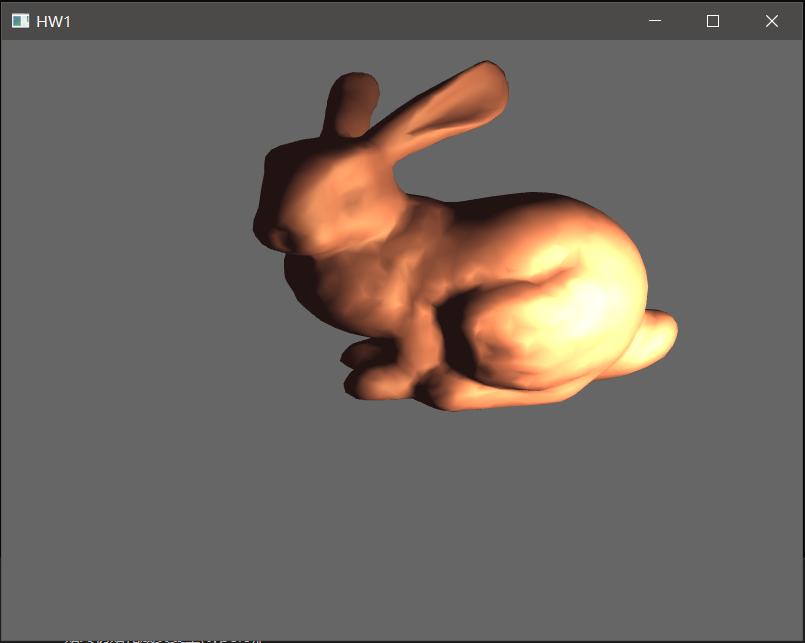
\includegraphics[width=4cm,height=5cm]{bunny.png}
\caption{Little cute bunny with warm light}
\end{figure}
The result is quite different to my expectation. The light result in many rough shadow with obvious lines on the model. Yet the result from my friend was quite smooth. But this can not be the Gouraud shading as I didn't do the linear interpolation on color. 


\end{document}
